\chapter{Camino Mínimo}

\section{Definición}

Dado un digrafo\footnote{Todos los algoritmos de camino mínimo que analizamos pueden ser fácilmente adaptados para operar en grafos no dirigidos.} pesado $G = (V, E, w)$, el peso de un camino $P$ entre sus vértices se define como la suma de los pesos de sus aristas:
$$w(P) = \sum_{e \in P} w(e)$$

Entonces, dados dos vértices $u$ y $v$, existe un camino de peso mínimo, es decir uno con el peso:
$$\delta(v, w) = \min{\{w(P) \mid P \text{ es un camino entre $v$ y $w$}\}}$$

La función $\delta(v, w)$ sigue reglas similares a $d(v, w)$, es decir:
\begin{itemize}
    \item $\delta(v, v) = 0\ \forall v \in V$
    \item $\delta(u, v) = \infty \iff \text{$u$ no es alcanzable desde $v$}$
\end{itemize}

$P$ es un \textit{camino mínimo} cuando $w(P) = \delta(v, w)$, y no necesariamente es único.

\begin{figure}[H]
    \centering
    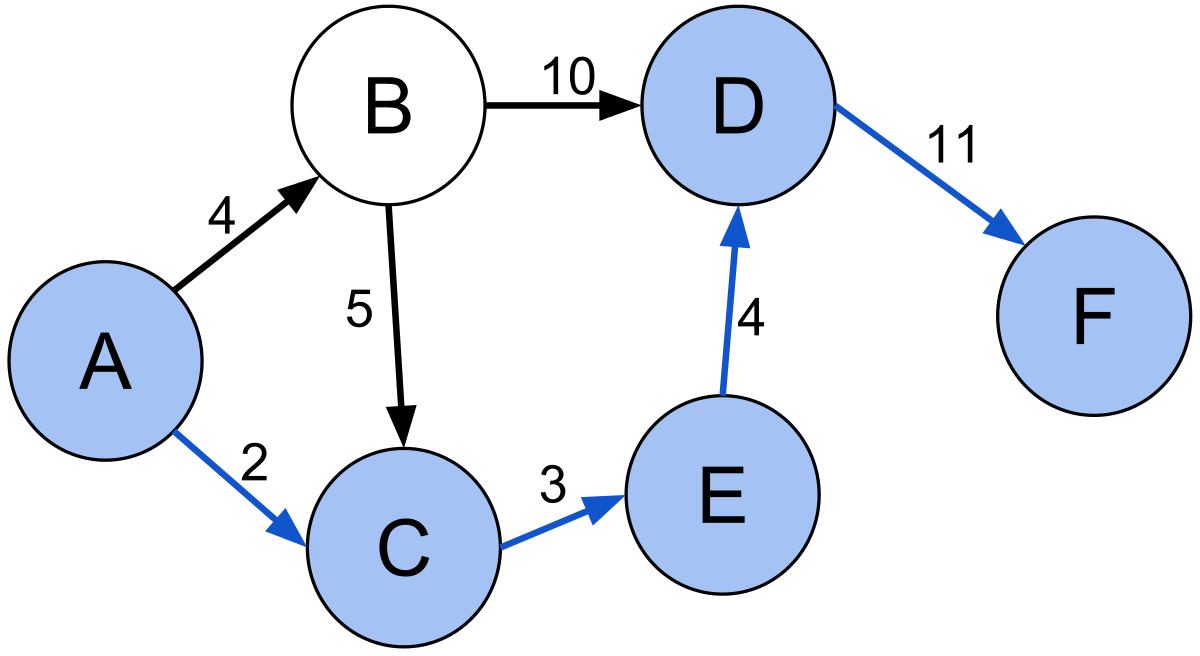
\includegraphics[width=0.5\textwidth]{ejemplo_camino_minimo.png}
    \caption*{El camino mínimo entre el par de vértices $A$ y $F$.}
\end{figure}

Este mínimo existe porque el conjunto de caminos es finito: a lo sumo hay $n!$, uno por cada permutación de los vértices de $G$. Esto no necesariamente vale en el caso de recorridos, que pueden tener vértices repetidos.

Un problema análogo es el de \textit{camino máximo}, que es el camino de peso máximo entre un par de vértices.

\subsection{Existencia}

A pesar de que un \textbf{camino} mínimo entre $u$ y $v$ siempre existen (asumiendo que están conectados), no es el caso para los recorridos: si un grafo tiene algún \textit{ciclo de peso negativo} (o simplemente \textit{ciclo negativo}) alcanzable desde $u$ y $v$, este puede ser transitado múltiples veces para obtener un peso tan bajo como se desee.

\subsection{Camino mínimo elemental}

El problema de esta índole más simple de definir (y más general) es el de \textit{camino mínimo elemental}:

\begin{problema}
    Dado un (di)grafo $G = (V, E, w)$ y un par de vértices $v, u \in V$, encontrar el camino (sin vértices repetidos) de peso mínimo.
\end{problema}

Como establecimos antes, este problema esta bien definido para cualquier grafo y cualquier par de vértices. El problema de \textit{camino máximo elemental}, donde se busca el camino de peso máximo, se puede reducir fácilmente a este: basta con tomar una función de peso $w'(e) = -w(e)$\footnote{A pesar de que los problemas son equivalentes, las aplicaciones de camino mínimo suelen ser en casos donde los pesos son no negativos (y por ende el grafo no tiene ciclos negativos). En tal caso, encontrar un camino máximo se vuelve más difícil, ya que negar los pesos hace que casi cualquier ciclo sea negativo. Es por esto que camino máximo se considera ``más difícil''.}.

Para el caso general, este problema es \hyperref[np-hard]{NP-hard}, así que se suelen estudiar casos restringidos. La restricción más importante para nuestros algoritmos es que el grafo no tenga ciclos negativos. En ese caso, encontrar un camino mínimo es equivalente a encontrar un recorrido mínimo.

\label{teorema-ciclos-negativos}
\begin{theorem*}
    Si un (di)grafo $G = (V, E, w)$ no tiene ningún ciclo negativo, existe un camino entre cualquier par de vértices $v, u \in V$ con peso total menor al de cualquier recorrido.
\end{theorem*}
\begin{proof}
    Supongamos que existe algún recorrido $R = v \cdots u$ que no es un camino y cuyo peso $w(R)$ es menor a la longitud de todos los caminos entre $v$ y $u$. Debido a que no es camino, tiene que pasar por dos veces por algún vértice $z$, definiendo un ciclo $R_{z_1 z_2}$\footnote{$z_1$ y $z_2$ no son vértices distintos, sino formas de distinguir las apariciones de $z$ en $R$.}. Como el grafo no tiene ciclos negativos, $w(P_{z_1 z_2}) \geq 0$, y entonces se puede definir un nuevo recorrido $R' = R_{v z_1} + R_{z_2 u}$ que ``recorta'' el ciclo, y cumple $w(R') = w(R) - w(R_{z_1 z_2}) \leq w(R)$. Este proceso puede repetirse hasta conseguir un camino de peso menor o igual al recorrido original, lo cual contradice la suposición inicial.
\end{proof}

\subsubsection{Subestructura óptima}

El problema de encontrar un camino mínimo $P_{uv}$ entre un par de vértices $u$ y $v$ cumple el \hyperref[optimalidad-bellman]{princpio de optimalidad de Bellman}: Cualquier subcamino $P_{u'v'} \subseteq P_{uv}$ es a su vez un camino mínimo entre $u'$ y $v'$.
\begin{theorem*}
    Dado un digrafo pesado $G = (V, E, w)$ sin ciclos negativos y un camino mínimo $P = v_1 \cdots v_k$, el subcamino $P_{v_i v_j}$ es un camino mínimo entre $v_i$ y $v_j$.
\end{theorem*}
\begin{proof}
    Supongamos que $P_{v_i v_j}$ no es un camino mínimo. Eso implica que existe un camino alternativo $P' = v_i \cdots v_j$ tal que $w(P') < w(P_{v_i v_j})$. En tal caso, se podría construir el recorrido $R = P_{v_1 v_i} + P' + P_{v_j v_k}$, para el cual existen dos posibilidades:
    \begin{itemize}
        \item Si el recorrido $R$ es un camino, entonces $w(R) = w(P_{v_1 v_i}) + w(P') + w(P_{v_j v_k}) < w(P_{v_1 v_i}) + w(P_{v_i v_j}) + w(P_{v_j v_k}) = w(P)$, lo cual es absurdo porque $P$ es un camino mínimo.
        \item Si el recorrido $R$ no es un camino, hay algún vértice $v_a$ por el que pasa 2 veces. Esto forma un ciclo $C = R_{v_{a1} v_{a2}}$ dentro del recorrido, que por hipótesis debe tener peso no negativo. Por lo tanto, si se ``recorta'' el ciclo, se obtiene un recorrido $R' = R_{v_1 v_{a1}} R_{v_{a2} v_k}$ de peso menor o igual. Estos recortes se pueden repetir hasta obtener un camino que, al igual que en el caso anterior, tiene peso estrictamente menor a $P$ (\textbf{Absurdo}).
    \end{itemize}

    Como ambas alternativas llevan a una contradicción, la suposición inicial ($P_{v_i v_j}$ no es camino mínimo) es falsa.
\end{proof}

\subsection{Árbol de caminos mínimos}

Ahora que definimos las restricciones necesarias (no hay ciclos negativos), se pueden empezar a analizar los métodos para encontrar caminos mínimos. Sorprendentemente, el problema de encontrar un camino mínimo entre $v$ y $u$ parece ser igual de difícil que el de encontrar el camino mínimo entre $v$ y todos los vértices del grafo, ya que no se conoce ningún algoritmo que resuelva el primero con una complejidad  de peor caso estrictamente menor a los métodos para resolver el otro.

Este nuevo problema se llama \textit{camino mínimo con un origen y múltiples destinos} (SSSP\footnote{\textit{Single Source Shortest Path.}}), y los caminos definen un árbol enraizado en $v$, llamado el \textit{árbol de caminos mínimos} (ACM). Un $v$-ACM es análogo a un árbol $v$-geodésico, solo que en este caso se cumple $\delta_T(v, u) = \delta_G(v, u)\ \forall u \in V$.

\section{Algoritmo de Dijkstra}

El \textit{algoritmo de Dijkstra} es uno de los más famosos en todo el área de computación. Este resuelve el problema de camino mínimo uno a todos, bajo la restricción de que los pesos de las aristas son no negativos.

\subsection{Definición}

El procedimiento general es similar al de Prim: se mantiene un árbol enraizado en el vértice inicial $v$ junto con una ``frontera'' de vértices adyacentes a los del árbol. En cada paso, se agrega el vértice de la frontera más cercano a la raíz. Esto puede ser clasificado como goloso, ya que en cada iteración se toma la decisión más ventajosa a corto plazo. Extendiendo la comparación, mientras que Prim agrega la arista segura de costo mínimo, Dijkstra agrega la que conecta al vértice con menor distancia a $v$.

\begin{codebox}
    \Procname{$\proc{Dijkstra}(G, w, s)$}
    \li $T \gets (V_T = \{s\}, E_T = \emptyset)$
    \li Inicializar arreglo $d$ con $+\infty$ en cada posición.
    \li $d[s] \gets 0$
    \li \For $i \gets 1$ \To $n - 1$ \Do
    \li $u \rightarrow v \gets \arg\min{\{d[x] + w(x \rightarrow y) \mid x \in V_T, y \in V - V_T\}}$
    \li $d[v] \gets d[u] + w(u \rightarrow v)$
    \li $V_T \gets V_T \cup \{v\}$
    \li $E_T \gets E_T \cup \{u \rightarrow v\}$
    \End
    \li \Return $(T, d)$
\end{codebox}

El diccionario $d$ contiene la distancia mínima entre $s$ y cada vértice. Esto se puede utilizar, entre otras cosas, para obtener el camino mínimo a cualquier vértice $u$ en tiempo lineal: se puede revisar el vecindario de entrada $N^-(u)$ hasta encontrar un vértice $v \in N^-(u)$ tal que $d[v] + w(v \rightarrow u) = d[u]$. Esto significa que hay un camino mínimo que pasa por la arista $v \rightarrow u$, y el proceso se puede repetir hasta llegar a $s$.

El algoritmo puede modificarse para grafos disconexos: debe mantener un conjunto de vértices conectados, y frenar cuando no quedan nuevos vértices por explorar. El comportamiento en ese caso es devolver los caminos mínimos a los vértices alcanzables (los demás están a distancia $\infty$).

\subsubsection{Generalización}

El procedimiento se puede generalizar para cualquier función $\bullet: \R \times \R \longrightarrow \R$ no decreciente de forma que el costo $w_\bullet(P)$ de un camino $P = v_1 \cdots v_k$ sea:
$$
    w_\bullet(v_1 \cdots v_k) =
    \begin{cases}
        0                                                    & \si k = 1 \\
        w_\bullet(v_1 \cdots v_{k-1}) \bullet c(v_{k-1} v_k) & \ecc
    \end{cases}
$$

La restricción de ser \textit{no decreciente} significa que $w_\bullet(P + y) \geq w_\bullet(P)$ para todo camino $P$ y vértice $y$. La suma cumple esto solo cuando los pesos son no negativos.

Si se define $\bullet$-peso de un camino $P$ al valor $w_\bullet(P)$, se puede llamar camino $\bullet$-mínimo al camino entre $v$ y $u$ con menor $\bullet$-peso (y $\delta_\bullet(v, u)$ al peso de ese camino). Más aún, el árbol de caminos $\bullet$-mínimos de $v$ es uno en el cual $\delta_{G,\bullet}(v, u) = \delta_{T, \bullet}(v, u)$ para todo $u$.

Finalmente, si se tiene un $\bullet$-ACM $T$ enraizado en $v$, se puede definir $w_\bullet(x \rightarrow v) = w_\bullet(P) \bullet w(x \rightarrow y)$, donde $P$ es el camino de $T$ entre $v$ y $x$. Esto permite diseñar el siguiente algoritmo general:

\begin{codebox}
    \Procname{$\proc{Dijkstra-$\bullet$}(G, w, s)$}
    \li $T \gets (V_T = \{s\}, E_T = \emptyset)$
    \li \For $i \gets 1$ \To $n - 1$ \Do
    \li $u \rightarrow v \gets \arg\min{\{w_\bullet(x \rightarrow y) \mid x \in V_T, y \in V - V_T\}}$
    \li $V_T \gets V_T \cup \{v\}$
    \li $E_T \gets E_T \cup \{u \rightarrow v\}$
    \End
    \li \Return $(T, d)$
\end{codebox}

Bajo esta definición, el algoritmo de Prim es solo una versión de \proc{Dijkstra-$\bullet$}, donde la función $\bullet(x, y)$ es $\max{\{x, y\}}$.

\subsection{Correctitud}

Se podría demostrar la correctitud de la función \proc{Dijkstra-$\bullet$}, pero para el final es más útil el caso particular de camino mínimo.

\begin{theorem*}
    Dado un (di)grafo pesado sin ciclos negativos $G = (V, E, w)$ y un origen $s \in V$, el algoritmo de Dijkstra devuelve un $s$-ACM $T$, y $d[u] = \delta(v, u)\ \forall u \in V$.
\end{theorem*}
\begin{proof}
    Se procede demostrando la siguiente hipótesis inductiva: para cada $0 \leq k \leq n - 1$, el grafo $T_k = (V_k, E_k)$ mantenido por Dijkstra en la $k$-ésima iteración es un árbol que cumple $\delta_{T_k}(s, u) = \delta_{G}(s, u)\ \forall u \in V_{k}$, y además $d[u] = \delta_{G}(s, u)\ \forall u \in V_{k}$.

    \textbf{Caso Base}: Antes de la primera iteración, $T_0 = (\{s\}, \emptyset)$, y se cumple que $d[s] = 0 = \delta(s, s)$ (por definición).

    \textbf{Paso Inductivo}: Llamemos $u \rightarrow v$ el arco que se agrega al árbol en la $k$-ésima iteración, es decir, $T_k = (V_k, E_k) = (V_{k - 1} \cup \{u\}, E_{k - 1} \cup \{u \rightarrow v\})$. Es claro que $T_k$ sigue siendo un árbol, ya que la nueva arista conecta a un vértice que no estaba en el grafo (y por ende no puede formar un ciclo).

    Sea $P = s \cdots y$ un camino mínimo entre $s$ e $y$, es decir, $w(P) = \delta(s, y)$. Tomamos el último vértice $x$ del camino que pertenece a $V_{k - 1}$, y sea $y$ el que lo sigue (estos deben existir, porque $x$ está en el conjunto, e $y$ no). Como se demostró anteriormente, $w(P_{su}) = \delta(s, u)$ (es subcamino de un camino mínimo). Como la arista $x \rightarrow y$ conecta un vértice de $V_{k - 1}$ con uno de $V - V_{k - 1}$, se debe cumplir que:
    \begin{flalign*}
         &  & d[u] + w(u \rightarrow v)         & \leq  d[x] + w(x \rightarrow y)        &  & \text{($u \rightarrow v$ fue elegida por Dijkstra)} \\
         &  & \delta(s, u) + w(u \rightarrow v) & \leq \delta(s, x) + w(x \rightarrow y) &  & \text{(Por HI, ya que $u, x \in T_{k - 1}$)}
    \end{flalign*}

    Entonces, se tiene que el camino une a $s$ con $v$ en $T_k$, $P'$ tiene un peso
    $$w(P') =
        \delta(s, u) + w(u \rightarrow v)
        \leq \delta(s, x) + w(x \rightarrow y)
        \underset{w \geq 0}{\leq} \underbrace{\delta(s, x) + w(x \rightarrow y) + w(P_{yv})}_{= w(P) \text{, que es un CM}}
        = \delta(s, v)$$

    Así que el camino $P'$ es mínimo, y $T_k$ cumple que las distancias de sus vértices son las mínimas en el grafo. Por otro lado, el nuevo valor de $d[v] = d[u] + w(u, v)$ es la distancia mínima de $s$ a $v$.

\end{proof}

\subsection{Complejidad}

La complejidad de Dijkstra es análoga a \hyperref[complejidad-prim]{la de Prim}: solo es necesario mantener un arreglo adicional con las distancias a cada nodo, lo cual no impone ningún costo en términos de tiempo. Por ende, el tiempo de ejecución dependerá de como se implemente la cola de prioridad de vértices a agregar:
\begin{itemize}
    \item \underline{Arreglo}: \BigO{|V|^2}.
    \item \underline{Binary Heap o AVL}: \BigO{|E|\log{|V|}}.
    \item \underline{Fibonacci Heap}: \BigO{|E| + |V|\log{|V|}}.
\end{itemize}

\section{Bellman-Ford}

El \textit{algoritmo de Bellman-Ford}, al igual que el de Dijkstra, resuelve el problema de camino mínimo de uno a todos. Sin embargo, a diferencia de este, Bellman-Ford puede ser utilizado en (di)grafos con pesos negativos (pero sin ciclos negativos). Si el grafo tiene algún ciclo alcanzable desde el vértice de origen, Bellman-Ford es capaz de detectarlo.

\subsection{Definición}

Este algoritmo se basa en ``\textit{relajar}'' las aristas del grafo. La relajación de $u \rightarrow v$ implica comprobar si el camino mínimo que va del origen a $v$ puede ser mejorado pasando por la arista. Si las distancias mínimas $\delta(s, v)$ se guardan en $d[v]$, se peude expresar de la siguiente manera:

\begin{codebox}
    \Procname{$\proc{Relajar}(u \rightarrow v, w)$}
    \li $d[v] \gets \min{\{d[u] + w(u \rightarrow v), d[v]\}}$
\end{codebox}

Bellman-Ford repite esta operación para cada arista, $|V| - 1$ veces. En cada iteración $i$ ciclo, los vértices se conectan a $s$ por caminos de a lo sumo $i$ aristas.

\begin{codebox}
    \Procname{$\proc{Bellman-Ford}(G, w, s)$}
    \li Inicializar arreglo de distancias $d$ con $+\infty$ en cada posición
    \li $d[s] \gets 0$
    \li \For $i \gets 0$ \To $n - 1$ \Do
    \li \For \Each $e \in E$ \Do
    \li $\proc{Relajar}(e, w)$
    \End
    \End
    \li \For \Each $u \rightarrow v \in E$ \Do
    \li \If $d[u] + w(u \rightarrow v) < d[v]$ \Then
    \li \Return Hay un ciclo negativo
    \End
    \End
    \li \Return $d$
\end{codebox}

El último ciclo chequea si existe algún ciclo negativo. Esto se debe a que, si alguna arista se puede relajar después de $i$ iteraciones, el recorrido más corto entre $s$ y algún vértice tiene $|V|$ aristas, lo cual implica que contiene un ciclo negativo (se demuestra más adelante).

El algoritmo puede adaptarse para devolver un $s$-ACM: basta con actualizar el padre de $v$ en \proc{Relajar}, es decir, asignar $prev[v] \gets u$.

\subsection{Correctitud}

Primero analizamos el caso de grafos sin ciclos negativos:

\begin{theorem*}
    Dado un (di)grafo pesado $G = (V, E, w)$ sin ciclos negativos, el algoritmo de Bellman-Ford devuelve en $d$ las distancias $d[v] = \delta(s, v)$.
\end{theorem*}
\begin{proof}
    Para demostrar esto, se demuestra la siguiente propiedad hipótesis inductiva: para cada iteración $k$ del ciclo exterior de Bellman-Ford, si un vértice $v$ está conectado a $s$ por un camino mínimo $P$ tal que $|P| \leq k$, se tiene que $d_{k}[v] = \delta(s, v)$, y $d_k[u] \geq \delta(s, u)\ \forall v \in V$.

    \textbf{Caso Base}: Para $k = 0$, el único vértice conectado por un camino de longitud $0$ es $s$, y se cumple que $d[s] = \delta(s, s) = 0$

    \textbf{Paso Inductivo}: Primero, demuestro la parte auxiliar de la hipótesis inductiva: sabiendo que $d_{k - 1}[u] \geq \delta(s, u)\ \forall v \in V$, se puede analizar la asignación de \proc{Relajar} (es el único procedimiento que cambia $d$ en el algoritmo):
    $$d_k[u] \gets \min{\{d_{k - 1}[u], d_{k - 1}[u'] + w(u' \rightarrow u)\}}$$

    Podemos ver que ambas opciones cumplen la propiedad: $d_{k - 1}[u] \geq \delta(s, u)$ por HI, mientras que: $d_{k - 1}[u'] + w(u' \rightarrow u) \geq \delta(s, u') + w(u' \rightarrow u) \geq \delta(s, u)$ (desigualdad triangular).

    Luego, por hipótesis sabemos que en el paso $k - 1$-ésimo se cumplía que $d_{k - 1}[v] = \delta(s, v)$ para cualquier vértice $v$ con camino mínimo de longitud menor o igual a $k - 1$. Esto se sigue cumpliendo en $d_k$ para esos mismos vértices gracias a que, como \proc{Relajar} asigna:
    $$d_k[v] \gets \min{\{d_{k - 1}[v], d_{k - 1}[u] + w(u \rightarrow v)\}}$$

    Se tiene que $d_k[v] \leq d_{k - 1}[v] = \delta(v, s)$. Como demostramos previamente, $d_k[v] \geq \delta(v, s)$, así que $d_k[v] = \delta(v, s)$.

    Por otro lado, para aquellos vértices $z$ tales que el camino mínimo de $s$ a $z$ es $P = s \cdots z$ de longitud $|P| = k$, sea $z'$ el anteúltimo vértice. Debido a que $P_{sz'} = s \cdots z'$ es también camino mínimo (es subcamino de un camino mínimo) y tiene longitud $k - 1$, sabemos por $HI$ que $d_{k - 1}[z'] = \delta(s, z')$. Esto, implica que $d_{k - 1}[z'] + w(z' \rightarrow z) = \delta(s, z') + w(z' \rightarrow z) = w(P) = \delta(s, z)$. Por lo tanto, en la asignación:
    $$d_k[z] \gets \min{\{d_{k - 1}[z], d_{k - 1}[z'] + w(z' \rightarrow z)\}}$$
    Como $d_{k - 1}[z] \geq \delta(s, z)$, se tiene $d_k = \delta(s, z)$.

    Finalmente, habiendo demostrado la inducción, nos sirve un caso particular de la misma: después de la última iteración, todos los vértices conectados al origen por un camino mínimo de longitud máxima $|V| - 1$ tendrán los pesos asignados de forma correcta. Estos son pesos son las distancias $\delta(s, v)$, porque en caso contrario el recorrido mínimo tendría que tener longitud mayor a $|V| - 1$, y por ende repetir algún vértice (esto \hyperref[teorema-ciclos-negativos]{no sucede} en grafos sin ciclos negativos).

\end{proof}

El comportamiento cuando hay ciclos negativos también es correcto:

\begin{theorem*}
    Si un (di)grafo pesado $G = (V, E, w)$ tiene algún ciclo de peso negativo $C$ alcanzable desde un origen $s$, el algoritmo de Bellman-Ford lo detecta.
\end{theorem*}
\begin{proof}
    Primero, demuestro la siguiente hipótesis inductiva: en la $k$-ésima iteración de relajaciones, cualquier vértice $u$ con distancia\footnote{Distancia es la longitud del camino más corto, no el peso del camino mínimo.} a $s$ menor o igual a $k$ cumple $d_k[v] < \infty$

    \textbf{Caso Base}: El único vértice alcanzable desde $s$ a través de $0$ aristas es $s$ en sí, y $d[s] = 0 < \infty$.

    \textbf{Paso inductivo}: Si la propiedad vale para $k - 1$, entonces $d_{k - 1}[u] < \infty$ para los $u$ a distancia $\leq k - 1$ de $s$. Después de la iteración $k$, eso se sigue cumpliendo para esos vértices, ya que \proc{Relajar} asigna un mínimo entre dos valores, uno de los cuales es $d_{k - 1}[u]$, así que $d_k[u] \leq d_{k - 1}[u] < \infty$.

    Por otro lado, si un vértice $u$ está a distancia $k$ de $s$, existe un camino $P = s \cdots u$ tal que $|P| = k$. Si llamamos $u'$ al anteúltimo vértice de $P$, se puede ver que $d_{k - 1}[u] < \infty$, ya que el camino $P_{su'}$ tiene longitud $k - 1$ (hipótesis inductiva). Luego, el valor $d_k[u]$ está dado por un mínimo entre dos valores, uno de los cuales es $d_{k - 1}[u'] + w(u' \rightarrow u) < \infty$ (es una suma de valores finitos), así que $d_k[u] < \infty$. Entonces, queda demostrado el caso $k$.

    En el caso particular de $k = |V| - 1$, cualquier vértice $v$ alcanzable desde $s$ tiene $d[v] < \infty$, ya que si existe un recorrido entre ambos, se pueden recortar los ciclos del mismo para obtener un camino (que tiene una longitud de a lo sumo $|V| - 1$).

    Sea $C = v_0 \cdots v_l$ el ciclo de peso negativo alcanzable desde $v$. Se tiene que:
    $$w(C) = \sum_{i = 1}^l w(v_{i - 1} \rightarrow v_i) < 0$$

    Supongamos que el algoritmo no detecta ningún ciclo. Esto implica que $d[u] + w(u \rightarrow v) < d[v]$ para todas las aristas del grafo. En particular, $d[v_i] \leq d[v_{i - 1}] + w(v_{i + 1} \rightarrow v_i)\ \forall i = 1 ... l$. Sumando estas desigualdades:
    \begin{align*}
        \sum_{i = 1}^l d[v_i] & \leq \sum_{i = 1}^l d[v_{i - 1}] + w(v_{i - 1} \rightarrow v_i)                \\
        \sum_{i = 1}^l d[v_i] & \leq \sum_{i = 1}^l d[v_{i - 1}] + \sum_{i = 1}^l w(v_{i - 1} \rightarrow v_i)
    \end{align*}

    Por otro lado, como $C$ es un ciclo, $v_0 = v_l$, y por ende:
    $$\sum_{i = 1}^k d[v_i] = \sum_{i = 0}^{k - 1} d[v_i] = \sum_{i = 1}^k d[v_{i - 1}]$$

    Como los vértices son alcanzables desde el origen, sus valores $d[v_i]$ son finitos, así que:
    \begin{align*}
        \sum_{i = 1}^l d[v_i]                               & \leq \sum_{i = 1}^l d[v_{i - 1}] + \sum_{i = 1}^l w(v_{i - 1} \rightarrow v_i) \\
        \sum_{i = 1}^l d[v_i] - \sum_{i = 1}^l d[v_{i - 1}] & \leq \sum_{i = 1}^l w(v_{i - 1} \rightarrow v_i)                               \\
        0                                                   & \leq \sum_{i = 1}^l w(v_{i - 1} \rightarrow v_i) = w(C)
    \end{align*}

    Esto es absurdo, así que el algoritmo tiene que haber detectado el ciclo.

\end{proof}

\subsection{Complejidad}

La complejidad de Bellman-Ford es fácil de calcular: \proc{Relajar} es una operación de tiempo constante, y corre $|E|$ veces en cada iteración (una por cada arista). Como hay $|V| - 1$ iteraciones, la complejidad es \BigO{|V||E|} (el último ciclo para comprobar la existencia de ciclos negativos es \BigO{|E|}, lo cual no cambia la complejidad).

\subsection{Mejoras}

% TODO

\subsection{Aplicación: Sistema de Restricciones de Diferencias}

Un problema que se puede resolver a través de Bellman-Ford es el de \textit{sistemas de restricciones de diferencias} (SRD). El enunciado es el siguiente:

\begin{problema}
    Encontrar un conjunto de valores $x_1, ..., x_n$, que respeten un sistema de $m$ inecuaciones de la forma:
    $$x_i - x_j \leq c_{ij}$$
\end{problema}

El problema se puede \hyperref[reducciones]{reducir} a camino mínimo el digrafo $D$, que tiene las siguiente características:
\begin{itemize}
    \item Para cada $i = 1, ..., n$, hay un vértice $v_i \in V_D$ que se corresponde con la incógnita $x_i$.
    \item Para cada inecuación $x_i - x_j \leq c_{ij}$, hay un arco $v_j \rightarrow v_i \in E_D$ de peso $w(v_j \rightarrow v_i) = c_{ij}$.
    \item Hay un vértice adicional $v_0$, que cuenta con arcos $v_0 \rightarrow v_i$ hacia todos los vértices $v_i$, todos de peso $w(v_0 \rightarrow v_i) = 0$.
\end{itemize}

El sistema tiene solución solo cuando el digrafo no tiene ciclos negativos

\begin{theorem*}
    Un sistema SRD tiene solución cuando el digrafo correspondiente $D$ no tiene ciclos negativos, y en tal caso la solución es $\{x_i = \delta(v_0, v_i) \mid 1 \leq i \leq n\}$.
\end{theorem*}
\begin{proof}
    Primero, veamos que pasa si $D$ tiene algún ciclo negativo $C = v_{i_0} \cdots v_{i_l}$. Supongamos que existe una solución $\{x_1, ..., x_n\}$. En tal caso, se tiene:
    $$\sum_{j = 1}^l w(v_{i_{j - 1}} \rightarrow v_{i_j}) = \sum_{j = 1}^l c_{i_j i_{j - 1}} < 0$$

    Si se suman las inecuaciones correspondientes del sistema, se llega a:
    \begin{align*}
        \underbrace{\sum_{j = 1}^l v_{i_j} - v_{i_{j - 1}}}_{\text{Suma telescópica}} & \leq \sum_{j = 1}^l c_{i_j i_{j - 1}} < 0 \\
        v_{i_l} - v_{i_0}                                                             & < 0
    \end{align*}

    Como $C$ es un ciclo, $v_{i_l} = v_{i_0}$, así que $0 < 0$ (\textbf{Absurdo}). Esto implica que no puede existir una solución para el sistema.

    Por otro lado, si no existe ningún ciclo de peso negativo, tomemos la asignación de valores $\{x_i = \delta(v_0, v_i) \mid 1 \leq i \leq n\}$. Entonces, para cada arco del grafo $v_j \rightarrow v_i$, se cumple la desigualdad triangular:
    $$\delta(v_0, v_i) \leq \delta(v_0, v_j) + w(v_j \rightarrow v_i)$$

    Reemplazando por los valores representados en el sistema,
    \begin{align*}
        x_i       & \leq x_j + c_{ij} \\
        x_i - x_j & \leq c_{ij}
    \end{align*}

    Es decir, se cumplen todas las desigualdades, así que $\{x_i = \delta(v_0, v_i) \mid 1 \leq i \leq n\}$ es una solución al sistema.

\end{proof}

Entonces, el sistema de ecuaciones se puede resolver encontrando el camino mínimo de un origen a todos los vértices o detectando algún ciclo de peso negativo alcanzable, que es precisamente lo que logra el algoritmo Bellman-Ford.

\section{Algoritmo de Floyd-Warshall}

\subsection{Definición}

El \textit{algoritmo de Floyd-Warshall} resuelve el problema de caminos mínimos todos a todos (APSP\footnote{All Pairs Shortest Paths}). Esto también se puede lograr corriendo alguno de los algoritmos anteriores (que devuelve el camino mínimo de uno a todos) para cada vértice, pero tendría desventajas: Dijkstra solo funciona cuando los pesos son no negativos, y $|V|$ ejecuciones  de Bellman-Ford sería (en general) más lento que este nuevo algoritmo. Al igual que antes, el grafo de entrada no puede tener ciclos de peso negativo.

Dado un grafo pesado $G = (V, E, w)$, se puede definir una matriz $L \in \R^{|V| \times |V|}$\footnote{Esto se puede considerar una extensión de la representación matriz de adyacencia, donde ahora cuando dos vértices están conectados por una arista se guarda su peso, y si no se guarda $\infty$.}, donde cada posición es el peso de la arista entre un par de vértices (si no existe una arista, el peso se considera infinito). Es decir,
$$
    l_{ij} =
    \begin{cases}
        0                      & \si i = j                     \\
        w(v_i \rightarrow v_j) & \si v_i \rightarrow v_j \in E \\
        \infty                 & \ecc
    \end{cases}
$$


El método calcula la \textit{matriz de distancias}, esto es, una matriz $D \in \R^{|V| \times |V|}$ tal que:
$$d_{ij} =
    \begin{cases}
        \delta(v_i, v_j) & \si \text{$v_i$ y $v_j$ están conectados} \\
        \infty           & \ecc
    \end{cases}$$

Para lograrlo, emplea la técnica de programación dinámica, empezando por $D^0 = L$, y calculando la siguiente matriz a través de la recurrencia:
$$d^k_{ij} = \min{\{d^{k - 1}_{ij}, d^{k - 1}_{ik} + d^{k - 1}_{kj}\}}$$

La matriz $D^k$ puede interpretarse como la matriz de distancias mínimas cuando se consideran solo los caminos que pasan por los vértices intermedios $\{v_1, ..., v_k\}$. Luego, después de $n$ iteraciones, la matriz $D^n$ es la matriz de distancias $D$.

El algoritmo se puede expresar de la siguiente manera:

\begin{codebox}
    \Procname{$\proc{Floyd-Warshall}(G)$}
    \li $D \gets L$
    \li \For $k = 1$ \To $|V|$ \Do
    \li \For $i = 1$ \To $|V|$ \Do
    \li \For $j = 1$ \To $|V|$ \Do
    \li $d_{ij} \gets \min{\{d_{ij}, d_{ik} + d_{kj}\}}$
    \End
    \End
    \End
    \li \Return $D$
\end{codebox}

En realidad, este algoritmo no implementa la recurrencia directamente: como utiliza una única matriz, hay casos en los que se asigna $d^k_{ij} = \min{\{d^{k - 1}_{ij}, d^k_{ik} + d^k_{kj}\}}$. Esto no afecta el resultado, solo tiene el efecto de converger más rápido a la matriz de distancias mínimas.

\subsection{Correctitud}

\begin{theorem*}
    Dado un (di)grafo pesado $G = (V, E, w)$ sin ciclos negativos, el algoritmo de Floyd-Warshall devuelve la matriz de distancias del mismo.
\end{theorem*}
\begin{proof}
    Para demostrar eso, primero demostramos por inducción que, en la iteración $k$ del ciclo exterior de FW, se cumple $d^k_{ij} = \delta(v_i, v_j)$ para cualquier par de vértices $v_i, v_j \in V$ conectados por un camino mínimo $P$ cuyos vértices intermedios están contenidos en $\{v_1, ..., v_k\}$ (es decir, $P \subseteq \{v_1, ..., v_k\} \cup \{v_i, v_j\}$). Además, se cumple para todos los vértices que $d^k_{ij} \geq \delta(v_i, v_j)$ (en todas las iteraciones).

    \textbf{Caso Base}: El caso base es $k = 0$. El conjunto de vértices intermedios sería $\emptyset$, y los únicos caminos mínimos sin vértices intermedios son aquellos constituidos por una sola arista. En esos casos, se cumple que $d^0_{ij} = w(v_i \rightarrow v_j) = \delta(v_i, v_j)$, gracias a que se asigna $D^0 \gets L$.

    Por otro lado, como asumimos que no hay ciclos de peso negativo, $\delta(v_i, v_i) = 0 = d^0_{ii} \forall i$, y para una arista $v_i \rightarrow v_j$ se tiene por desigualdad triangular:
    $$d^0_{ij} = w(v_i \rightarrow v_j) = \underbrace{{\delta(v_i, v_i)}}_{= 0} + w(v_i \rightarrow v_j) \geq \delta(v_i, v_j)$$

    \textbf{Paso Inductivo}: Supongamos que la propiedad vale en el caso $k - 1$. Recordemos que la asignación que se realiza en la iteración $k$ es:
    $$d^k_{ij} = \min{\{d^{k - 1}_{ij}, d^{k - 1}_{ik} + d^{k - 1}_{kj}\}}$$

    Para demostrar que $d^k_{ij} \geq \delta(v_i, v_j)$, notemos dos cosas:
    \begin{itemize}
        \item $d^{k - 1}_{ij} \geq \delta(v_i, v_j)$, por HI.
        \item $d^{k - 1}_{ik} + d^{k - 1}_{kj} \geq \delta(v_i, v_k) + \delta(v_k, v_j) \geq \delta(v_i, v_j)$, por HI y desigualdad triangular, respectivamente.
    \end{itemize}

    En todo caso, se cumple que $d^k_{ij} \geq \delta(v_i, v_j)$.

    Para los pares de vértices con caminos mínimos formados por vértices intermedios en el conjunto $\{v_1, ..., v_{k - 1}\}$, se sigue cumpliendo la propiedad, ya que la HI implica que $d^{k - 1}_{ij} = \delta(v_i, v_j)$ (así que $d^k_{ij} \leq \delta(v_i, v_j)$), y como recién demostramos que $d^k_{ij} \geq \delta(v_i, v_j)$, se tiene $d^k_{ij} = \delta(v_i, v_j)$.

    Por otro lado, sea $P = v_x \cdots v_y$ algún camino mínimo entre $v_x$ y $v_y$ que contiene al vértice $v_k$ y cuyos vértices intermedios están contenidos en $\{v_1, ..., v_k\}$. $P$ se puede descomponer como la concatenación $P_{v_x v_k} + P_{v_k v_y}$, y estos dos subcaminos (que son mínimos) están formados por vértices intermedios del conjunto $\{v_1, ..., v_{k - 1}\}$ (si estuviera $v_k$ en el medio, aparecería dos veces, y no serían caminos simples). Esto, por HI, implica que $d^{k - 1}_{xk} = \delta(v_x, v_k) = w(P_{v_x v_k})$ y $d^{k - 1}_{ky} = \delta(v_k, v_y) = w(P_{v_k v_y})$, así que cuando se asigna:
    $$d^k_{ij} = \min{\{d^{k - 1}_{ij}, d^{k - 1}_{ik} + d^{k - 1}_{kj}\}}$$

    Se obtiene $d^k_{xy} \leq d^{k - 1}_{xk} + d^{k - 1}_{ky} = w(P_{v_x v_k}) + w(P_{v_k v_y}) = w(P) = \delta(v_x, v_y)$ que, junto con $d^k_{xy} \geq \delta(v_x, v_y)$ (se demostró previamente), significa que $d^k_{xy} = \delta(v_x, v_y)$. Queda demostrado entonces que la propiedad vale para el caso $k$.

    Como, por inducción, la propiedad se cumple después de cualquier iteración $k$, se cumple en particular para después de la última, lo cual significa que todo par de vértices $v_i, v_j$ conectado por un camino mínimo con vértices intermedios en $\{1, ..., v_{|V|}\} = V$ cumple $d^k_{ij} = \delta(v_i, v_j)$. Esto incluye a cualquier par de vértices conectados, y para los vértices que no son alcanzables entre sí, la segunda propiedad garantiza que $d^k_{ij} \geq \delta(v_i, v_j) = \infty \implies d^k_{ij} = \infty$. Por ende, todas las distancias de $D^{|V|}$ son correctas.

\end{proof}

\subsection{Complejidad}

La complejidad de Floyd-Warshall es fácil de calcular: tiene 3 ciclos anidados, de $|V|$ iteraciones cada uno, en cuyo interior se realizan operaciones de tiempo constante, así que el algoritmo es \BigO{|V|^3}. Como se mencionó previamente, esto es mejor que correr $n$ veces Bellman-Ford, siempre que el grafo sea conexo (porque en ese caso $|E| \geq |V| - 1 \implies |E| \in \BigOmega{|V|}$).

Una posible mejora sería chequear en cada iteración si $d_{ii} < 0$ para algún $i$, ya que esto implica que el grafo tiene un ciclo negativo (en el teorema anterior se demuestra $d_{ii} \geq \delta(v_i, v_i) = 0$ cuando no hay ciclos negativos), y cortar la ejecución.

\section{Camino Mínimo en DAGs}

\subsection{Definición}

Para el caso de digrafos acíclicos, camino mínimo uno a muchos puede resolverse utilizando un algoritmo más eficiente que los anteriores. Este se basa en la siguiente fórmula para la distancia entre dos nodos:
$$
    \delta(u, v) =
    \begin{cases}
        0                                                             & \si u = v \\
        \min{\{\delta(u, z) + w(z \rightarrow v) \mid z \in N^-(v)\}} & \ecc
    \end{cases}
$$

Esto es intuitivo: la distancia mínima entre un par de nodos $u, v$ es el peso de algún camino mínimo $P = u \cdots v$. El anteúltimo vértice del camino $z$ está en el vecindario de entrada de $v$ (ya que tiene una arista que apunta hacia él), mientras que el subcamino $P_{uz}$ también es mínimo.

Esta relación no se puede utilizar para computar las distancias en un grafo con un ciclo $C = v \cdots v$, ya que la llamada $\delta(u, v)$ llevaría a un bucle de recursión infinita (porque existe un camino de $v$ a $v$ a través de los vecindarios de entrada).

\subsubsection{Versión Top-Down}

La fórmula se puede implementar como un algoritmo de programación dinámica top-down. Asumiendo que el arreglo de distancias (que funciona estructura de memoización) $D$ se inicializa con $\perp$ en todas las posiciones, el código es el siguiente:

\begin{codebox}
    \Procname{$\proc{SP-DAG-Top-Down}(G, s, v)$}
    \li \If $s == v$ \Then
    \li \Return $0$
    \End
    \li \If $D[v] ==\ \perp$ \Then
    \li $D[v] \gets \min{\{\proc{SP-DAG-Top-Down}(G, s, z) + w(z \rightarrow v) \mid z \in N^-(v)\}}$
    \End
    \li \Return $D[v]$
\end{codebox}

\subsubsection{Versión Bottom-Up}

Esto también se puede implementar de forma bottom-up: las distancias son calculadas en \hyperref[orden-topologico]{orden topológico}, lo cual asegura que $D[z]$ es calculado antes de $D[v]$ para cualquier $z \in N^-(v)$\footnote{Esto se debe a que, en un orden topológico, los vértices $v$ que son alcanzables desde $z$ aparecen después en la secuencia}.

\begin{codebox}
    \Procname{$\proc{SP-DAG-Bottom-Up}(G, s)$}
    \li Inicializar arreglo de distancias $D$.
    \li Calcular un orden topológico de $G$.
    \li \For \Each $v \in V$, en orden topológico \Do
    \li \If $s == v$ \Then
    \li $D[v] \gets 0$
    \li \Else
    \li \If $N^-(v) \neq \emptyset$ \Then
    \li $D[v] \gets \min{\{D[z] + w(z \rightarrow v) \mid z \in N^-(v)\}}$
    \li \Else 
    \li $D[v] \gets \infty$
    \End
    \li \Return $D$
\end{codebox}

\subsection{Complejidad}

Ambos métodos tienen una complejidad \BigO{|V| + |E|} ya que pasan $1$ vez por cada nodo $v$, realizando una operación \BigO{d^-(v)}. En el caso bottom-up, se realiza el paso adicional de computar un orden topológico, pero esto también se puede realizar en tiempo lineal a través de DFS.

\section{Algoritmo de Johnson}

\subsection{Definición}

El algoritmo de Johnson resuelve el problema de camino mínimo todos a todos. Es una alternativa al algoritmo de Floyd-Warshall, y es más eficiente para grafos ralos. La idea general del método es ``repesar'' las aristas del grafo, de forma que todos los pesos nuevos sean no negativos y se preserven los caminos mínimos, para luego aplicar el algoritmo de Dijkstra en cada nodo.

El proceso de repesar se basa en el siguiente teorema:

\begin{theorem*}
    Dado un (di)grafo pesado $G = (V, E, w)$ y una función $h: V \longrightarrow \R$, se puede definir una nueva función de peso:
    $$\hat{w}(u \rightarrow v) = w(u \rightarrow v) + h(u) - h(v)$$

    Luego, si se toma el grafo ``repesado'' $\hat{G} = (V, E, \hat{w})$, cualquier camino mínimo $P$ en $G$ sigue siendo mínimo en $\hat{G}$, y $G$ tiene un ciclo negativo $\iff$ $\hat{G}$ tiene un ciclo negativo.
\end{theorem*}
\begin{proof}
    Dado un recorrido cualquiera $P = \langle v_0, ..., v_k \rangle$ se puede ver que:
    \begin{align*}
        \hat{w}(P) & = \sum_{i=1}^k \hat{w}(v_{i - 1}, v_i)                                                                       \\
                   & = \sum_{i=1}^k w(v_{i - 1}, v_i) + h(v_{i - 1}) - h(v_i)                                                     \\
                   & = \sum_{i=1}^k w(v_{i - 1}, v_i) + \underbrace{\sum_{i=1}^k h(v_{i - 1}) - h(v_i)}_{\text{Suma telescópica}} \\
                   & = \sum_{i=1}^k w(v_{i - 1}, v_i) + h(v_0) - h(v_k)                                                           \\
                   & = w(P) + h(v_0) - h(v_k)
    \end{align*}

    Por ende, si $P'$ es un camino mínimo entre $u$ y $v$ en $G$, se tiene:
    \begin{flalign*}
         &  & w(P')                & \leq w(P)               &  & \forall P \text{ camino entre $u$ y $v$} \\
         &  & w(P')  + h(u) - h(v) & \leq w(P) + h(u) - h(v) &  & \forall P \text{ camino entre $u$ y $v$} \\
         &  & \hat{w}(P')          & \leq \hat{w}(P)         &  & \forall P \text{ camino entre $u$ y $v$}
    \end{flalign*}

    Entonces, $P'$ sigue siendo camino mínimo en $\hat{G}$.

    Por otro lado, dado un ciclo $C = u \cdots u$, su peso en $\hat{G}$ es $\hat{w}(C) = w(C) + h(u) - h(u) = w(C)$, así que $\hat{G}$ tiene ciclos negativos si y solo si $G$ los tiene.

\end{proof}

Para aprovechar este resultado, hace falta encontrar una función $h: V \longrightarrow \R$ que permita asignar valores no negativos a todos los pesos. El algoritmo de Johnson logra esto agregando un vértice adicional $s$ a $G$, conectado a todos los vértices con aristas de peso $0$, y calculando las distancias mínimas de $s$ a los demás (a través del algoritmo de Bellman-Ford, acá es donde el procedimiento falla si hay un ciclo negativo). Luego, toma $h(v) = \delta(s, v)$, que resulta en pesos no negativos ya que:
\begin{flalign*}
     &  & \delta(s, v) & \leq \delta(s, u) + w(u \rightarrow v) &  & \text{(Desigualdad triangular)} \\
     &  & h(v)         & \leq h(u) + w(u \rightarrow v)         &  &                                 \\
     &  & 0            & \leq w(u \rightarrow v) + h(u) - h(v)  &  &                                 \\
     &  & 0            & \leq \hat{w}(u \rightarrow v)          &  &
\end{flalign*}

Luego, se puede correr Dijkstra en cada vértice para obtener las distancias de todos a todos. El código es el siguiente:

\begin{codebox}
    \Procname{$\proc{Johnson}(G, w)$}
    \li $G' \gets (V \cup \{s\}, E \cup \{s \rightarrow v \mid s \in E\})$, $w(s, v) = 0\ \forall v \in V$
    \li \If $\proc{Bellman-Ford}(G', w, s)$ encuentra un ciclo negativo \Then
    \li \Return Hay un ciclo negativo
    \li \Else \proc{Bellman-Ford} devolvió las distancias $\delta(s, v)\ \forall v \in V$.
    \li Definir $\hat{w}(u \rightarrow v) \gets w(u \rightarrow v) + \delta(s, u) - \delta(s, v)\ \forall u \rightarrow v \in E$.
    \li Inicializar matriz $D \in \R^{|V| \times |V|}$
    \li \For \Each $u \in V$ \Do
    \li Correr $\proc{Dijkstra}(G, \hat{w}, u)$ para obtener $\hat{\delta}(u, v)\ \forall v \in V$
    \li Asignar $d_{uv} \gets \hat{\delta}(u, v) - \delta(s, v) + \delta(s, u)\ \forall v \in V$
    \End
    \li \Return $D$
    \End
\end{codebox}

\subsection{Complejidad}

La ejecución del algoritmo de Johnson se divide en dos partes. Primero, se ejecuta Bellman-Ford en el vértice agregado $s$, lo cual tiene una complejidad de \BigO{|V||E|}. Luego, se corre el algoritmo de Dijkstra una vez en cada vértice, y el tiempo de ejeución de eso depende de la cola de prioridad que utilice ese procedimiento. Si se utiliza un Fibonacci heap, la complejidad de Dijkstra es \BigO{|V|\log{|V|} + |E|}, así que la complejidad total de Johnson es \BigO{|V|^2\log{|V|} + |V||E|}.
